%NAME: Thales circle thm proof gr.svg
\documentclass[tikz]{standalone}
\usepackage{pgfplots}
\pgfplotsset{compat=1.15}
\usepackage{mathrsfs}
\usetikzlibrary{arrows,calc}
\usepackage{tkz-euclide}
\pagestyle{empty}

\definecolor{AngleClr}{rgb}{0,0.39215686274509803,0}
\definecolor{ShapeClr}{rgb}{0.6,0.2,0}

\begin{document}

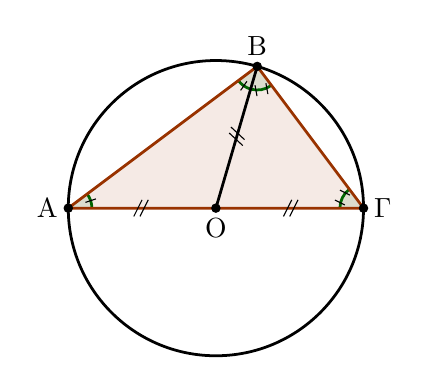
\begin{tikzpicture}[scale=.75]
\tkzSetUpLine[line width=1pt,color=black]
\tkzSetUpPoint[fill=black]

\tkzDefPoints{0/0/A,3.2/2.4/B,5/0/C,2.5/0/O}
\tkzDrawCircle[line width=1pt,color=black](O,A)

\tkzFillPolygon[fill=ShapeClr,fill opacity=0.1](B,A,C)
\tkzFillAngles[fill=AngleClr,size=.4,fill opacity=0.1](C,A,B A,B,O B,C,A O,B,C)
\tkzMarkAngles[mark=|,mksize=2,line width=1pt,size=.4,color=AngleClr](C,A,B A,B,O)
\tkzMarkAngles[mark=||,mksize=2,line width=1pt,color=AngleClr,size=.4](B,C,A O,B,C)

\tkzDrawPolygon[color=ShapeClr](A,B,C)
\tkzDrawPoints[size=3](A,B,C,O)
\tkzLabelPoint[left](A){$\rm A$}
\tkzLabelPoint[above](B){$\rm B$}
\tkzLabelPoint[right](C){$\rm \Gamma$}
\tkzLabelPoint[below](O){$\rm O$}

\tkzDrawSegment(O,B)

\tkzMarkSegments[mark=s||,size=3](O,A O,B O,C)

\end{tikzpicture}

\end{document}
